%%\title{APERTURE AND TOLERANCES}
%  Changed by: Mark HAYES, 19-Sep-2002 

%  Changed by: Ivar Waarum, 24-Feb-2005 

%%\usepackage{hyperref}
% commands generated by html2latex


%%\begin{document}
%%\begin{center}
 %%EUROPEAN ORGANIZATION FOR NUCLEAR RESEARCH 
%%\includegraphics{http://cern.ch/madx/icons/mx7_25.gif}

\subsection{Defining aperture in MAD-X}
%%\end{center}  A new feature of MAD-X is the ability to set an aperture for a particular  element, or parent of a set of elements. This removes the need of placing a collimator next to every element to do aperture tracking.  The aperture of any elements can be specified (excepts drifts) by the use of the following parameters: 
\begin{itemize}
	\item \texttt{APERTYPE} This can have seven text values: CIRCLE, RECTANGLE, ELLIPSE, LHCSCREEN (a superposition of a CIRCLE and a RECTANGLE), MARGUERITE (two LHCSCREENS, one rotated by 90 degrees),  RECTELLIPSE (a superposition of an ELLIPSE and a RECTANGLE) and RACETRACK. 
	\item \texttt{APERTURE} This is an array of values, the number and meaning  of which depends on the APERTYPE: 
\end{itemize}
%http://en.wikibooks.org/wiki/LaTeX/Tables#Text_wrapping_in_tables
\begin{tabular}{l | l | p{9cm}|}
\hline 
\textbf{APERTYPE} & \textbf{\# of parameters} & \textbf{meaning of parameters} \\ 
\hline
CIRCLE & 1 &  radius \\ 
\hline
ELLIPSE & 2 & horizontal half axis, vertical half axis \\ 
\hline
RECTANGLE & 2 & half width and half height \\ 
\hline
LHCSCREEN & 3 & half width, half height (of rect.) and radius (of circ.) \\ 
\hline
MARGUERITE & 3 & half width, half height (of rect.) and radius (of circ.) \\ 
\hline
RECTELLIPSE & 4 & half width, half height (of rectangle), horizontal half axis, vertical half axis (of ellipse) \\ 
\hline
RACETRACK & 3 & horizontal [1] and vertical [2] positions of the circle, radius [3] of the circle (see s, g, r in the figure below) \\ 
\hline
FILENAME & 0 & where the file contains a list of x and y coordinates outlining the shape. This option is only supported by the aperture module, see below. \\ 
\hline

\end{tabular}
  Here is an example for setting an ELLIPTICAL aperture for the main dipoles for the LHC. 
\begin{verbatim}

MB : SBEND, L := l.MB, APERTYPE=ELLIPSE, APERTURE={0.02202,0.02202};
\end{verbatim} And an example for setting a FILENAME aperture for another magnet. Notice that no aperture parameters are needed. 
\begin{verbatim}

MB: SBEND, L := 5, APERTYPE=myfile;
\end{verbatim} The syntax of myfile should be like this: 
\begin{verbatim}

x0   y0
xi   yi
...
xn   yn
\end{verbatim}  Notes concerning the use of aperture: 
\begin{itemize}
	\item There is some inconsistency in the parameter definition for the different APERTYPE. This is historical and has to be kept for backwards compatibility. Pay some attention to the parameters you introduce!
	\item When \href{../makethin/makethin.html}{MAKETHIN} is called all the  thin slices inherit the aperture from their original thick lens version. 
	\item When the SIXTRACK command is called (see the SixTrack converter module \href{../c6t/c6t.html}{C6T}) the apertures are ignored by default. To convert the apertures as well the APERTURE flag has to be set. 
	\item  Aperture parameters are like all parameters and are inherited by offspring. Like other parameters they can also be overridden by the offspring elements if necessary. 
\end{itemize}  The APERTYPE and the APERTUREs themselves can be conveniently added to the TWISS table (see \href{../twiss/twiss.html}{Twiss Module}) by using the \href{select.html}{SELECT} command. E.G. the command:  
\begin{verbatim}

select,flag=twiss,clear;
select,flag=twiss,column=name,s,betx,alfx,mux,bety,alfy,muy,apertype,
aper_1,aper_2;
\end{verbatim} and a subsequent TWISS command will put the aperture information together with the specified TWISS parameters into the TWISS table.  
%%\begin{center}


\subsection{Defining tolerances in MAD-X}
%%\end{center}
 A parameter closely connected to the aperture is the sum of the mechanical and alignment tolerances. The mechanical tolerance is the maximal error margin of errors in the element body which causes a decrease of aperture, and the alignment tolerance is a mislignment of the element in the accelerator, which also causes a decrease of aperture. The tolerance is given in the transverse plane as a racetrack, like in the picture below.
\\
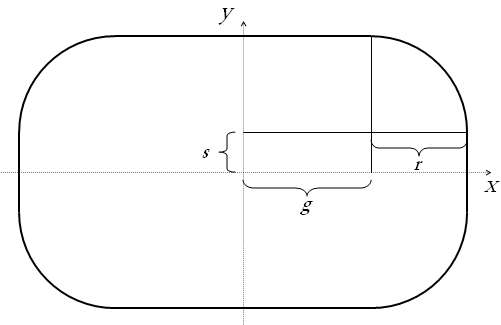
\includegraphics[width=450px]{Introduction/tolerance.jpg}%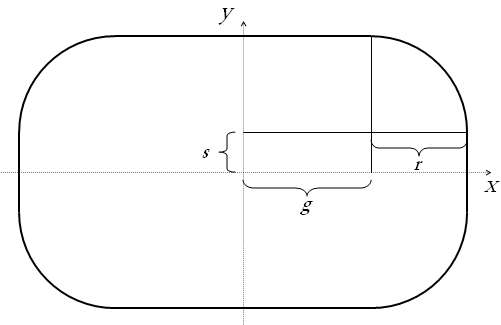
\includegraphics{Introduction/tolerance.jpg align=center width=450}
\\ A tolerance can be assigned to each element in a MAD-X sequence as a vector: 
\begin{verbatim}

Syntax: APER_TOL = {r, g, s};

MB : SBEND, L := l.MB, APER_TOL={1.5, 1.1, 0};
\end{verbatim}
%%\begin{center}


\subsection{APERTURE MODULE}
%%\end{center} 
Computes the n1 values for a piece of machine. Each element is sliced into thick subelements at given intervals, and the available aperture is computed at the end of each slice. The computation is based on the last Twiss table, so it is important to run the \href{../twiss/twiss.html}{Twiss} and aperture commands on the same period or sequence, see the aperture example below. Also showed in the example is how n1 values can be \href{../plot/plot.html}{plotted}.  

 The minimum n1 for each element is written to the last Twiss table, to allow for \href{../match/match.html}{matching} by aperture.  
\begin{itemize}
	\item 

%\paragraph{Aperture,}
\textbf{Aperture,}
\begin{verbatim}
file=filename,
halofile=filename,
pipefile=filename,
range=range,
exn=real,
eyn=real,
dqf=real,
betaqfx=real,
dp=real,
dparx=real,
dpary=real,
cor=r,
bbeat=real,
nco=integer,
halo={real,real,real,real},
interval=real
spec=real,
notsimple=logical,
trueprofile=filename,
offsetelem=filename;
\end{verbatim} where the parameters have the following meaning: 
\begin{itemize}
	\item file: Output file with aperture table. Default = none 
	\item halofile: Input file with halo polygon coordinates. Will suppress  an eventual halo parameter. Default = none 
	\item range: \href{../Introduction/ranges.html}{Range} given by  elements. Default = \#s/\#e 
	\item exn: Normalised horizontal emittance. Default = 3.75*e-6 
	\item eyn: Normalised vertical emittance. Default = 3.75*e-6 
	\item dqf: Peak linear dispersion [m]. Default = 2.086 
	\item betaqfx: Beta x in standard qf [m]. Default = 170.25 
	\item dp: Bucket edge at the current beam energy. Default = 0.0015 
	\item dparx: Fractional horizontal parasitic dispersion. Default = 0.273 
	\item dpary: Fractional vertical parasitic dispersion. Default = 0.273 
	\item cor: Maximum radial closed orbit uncertainty [m]. Default = 0.004 
	\item bbeat: Beta beating coefficient applying to beam size. Default = 1.1 
	\item nco: Number of azimuth for radial scan. Default = 5 
	\item halo: Halo parameters: \{n, r, h, v\}. n is the radius of the primary halo,  r is the radial part of the secondary halo, h and v is the horizontal and  vertical cuts in the secondary halo. Default = \{6, 8.4, 7.3, 7.3\} 
	\item interval: Approximate length in meters between measurements. Actual value:  nslice = nodelength/interval, nslice is rounded down to closest integer,  interval = nodelength/nslice. Default = 1.0 
	\item spec: Aperture spec, for plotting only. Gives the spec line in the plot. Default = 0.0 
	\item notsimple: Use only if one or more beamscreens in the range are considered not to  be a "simply connex". Since all MAD-X apertypes are simply connex, this is only possible  if an input file with beam screen coordinates are given. See below for a graphical example. Default = false. 
	\item trueprofile: A file containing a list of magnets, and for each magnet a list of horizontal and vertical deviations from the ideal magnet axis. These values may come from measurements done on the magnet. See below for example. Default = none. 
	\item offsetelem: A file containing a reference point in the machine, and a list of magnets with their offsets from this point described as a parabola. See below for example. Default = none. 
\end{itemize}



\subsubsection{Not simply connex beam pipes} Methodically, the algorithm for finding the largest possible halo is fairly simple. The distance from halo centre to the first apex (i = 0) in the halo is calculated (l\_i), and the equation for a line going through these points is derived. This line is then compared with all lines making the pipe polygon to find their respective intersection coordinates. The distance h\_i between halo centre and intersection are then divided by l\_i, to find the maximal ratio of enlargement, as seen below. This procedure is then repeated for all apexes i in the halo polygon, and the smallest ratio  of all apexes is the maximal enlargement ratio for this halo to just touch the pipe at this particular longitudinal position.
\\
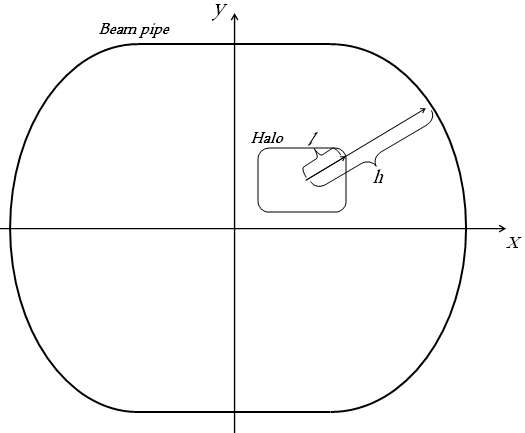
\includegraphics[width=420px]{Introduction/notsimple0.jpg}%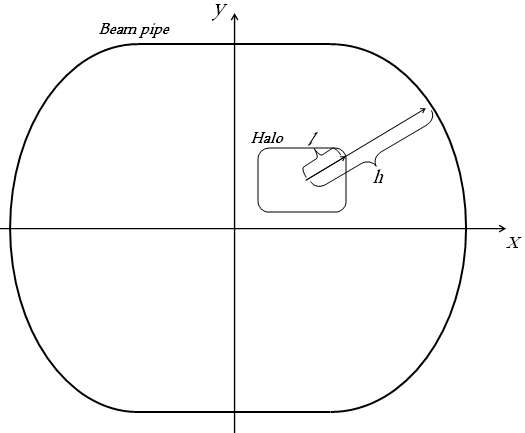
\includegraphics{notsimple0.jpg align=center width=420}
\\  There is one complication to this solution; polygons which are not simple connexes. (Geometrical definition of ``simply connex'': A figure in which any two points can be connected by a line segment, with all points on the segment inside the figure.) The figure below shows what happens when a beam pipe polygon is not a simple connex. The halo is expanded in such a way that it overlaps the external polygon in the area where the latter is dented inwards.
\\
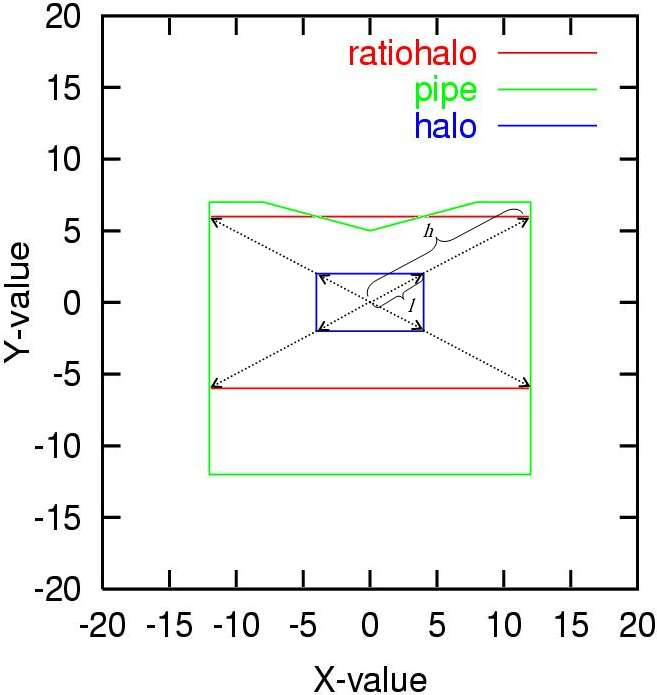
\includegraphics[width=420px]{Introduction/notsimple1.jpg}%%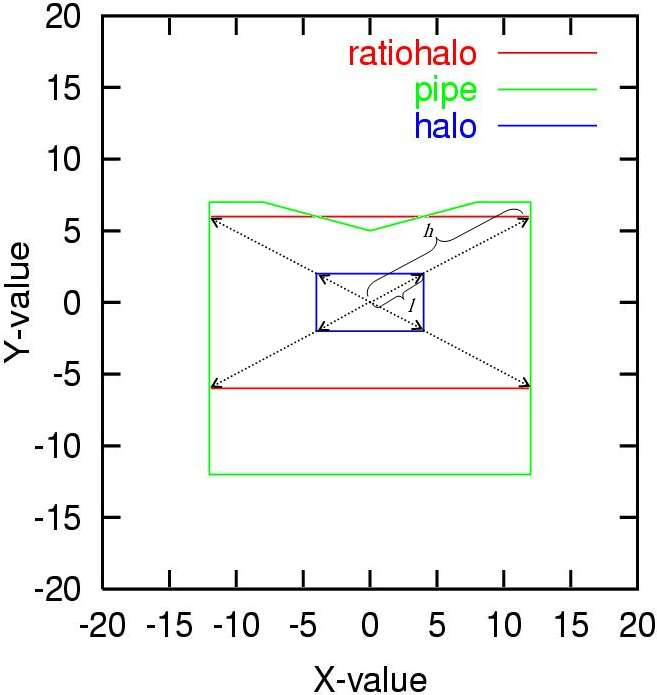
\includegraphics{notsimple1.jpg align=center width=420}
\\  To make the module able to treat all kinds of polygons, \textit{notsimple} must be activated. With this option activated, apexes are strategically added to the halo polygon wherever the beam pipe polygon might have an inward dent. This is done by drawing a line from halo centre to each apex on the pipe polygon. An apex with its coordinates on the intersection point line-halo is added to a table of halo polygon apexes. The result is that the halo polygon has a few ``excessive'' points on straight sections, but the algorithm used for expansion will now never miss a dent in the beam pipe. The use of the notsimple option significantly increases computation time.
\\
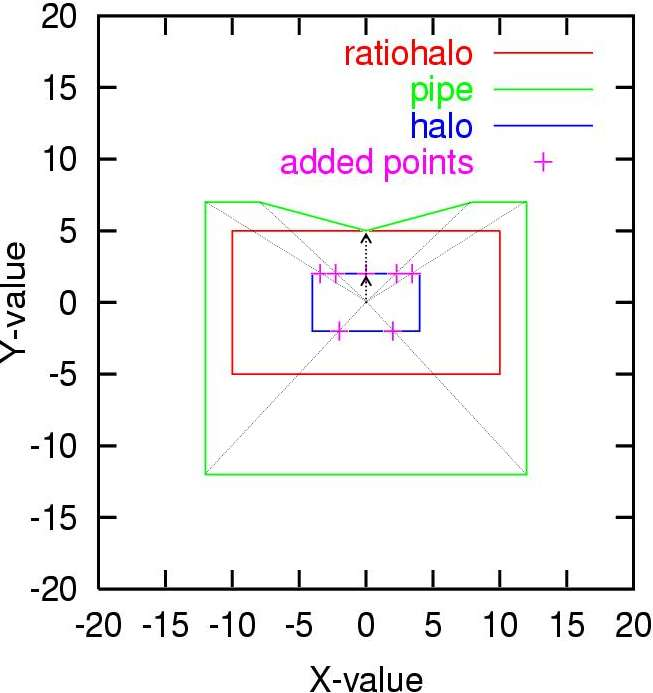
\includegraphics[width=420px]{Introduction/notsimple2.jpg}%%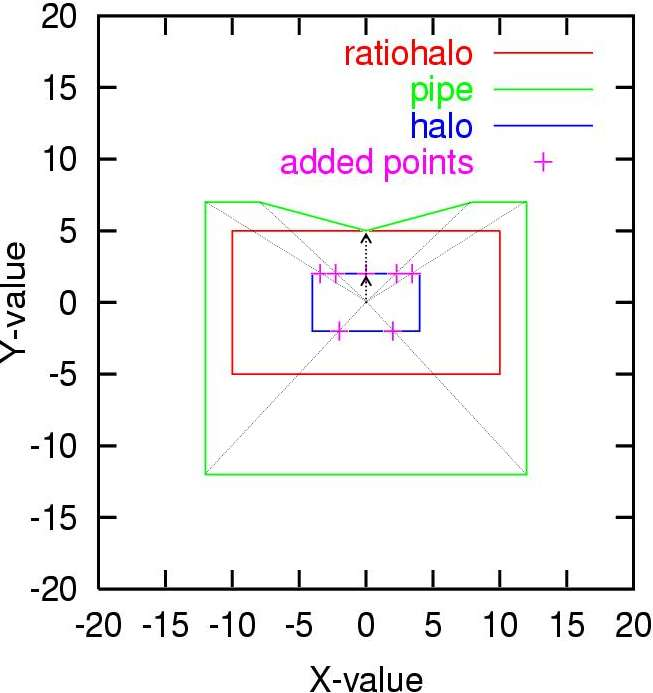
\includegraphics{notsimple2.jpg align=center width=420}
\\

\subsubsection{Trueprofile file syntax} This file contains magnet names, and their associated displacements of the axis for  an arbitrary number of S, where So is the start of the magnet and Sn the end. The interval between each S must be regular, and X and Y  must be given in meters. The magnet name must be identical to how it appears in the  sequence. The displacements are only valid for this particular magnet, and cannot be  assigned to a family of magnets. n1 is calculated for a number of slices determinated by the number of Si.
\\
\\

\subparagraph{Layout of file:}
\begin{verbatim}

magnet.name1
So   X   Y
Si   X   Y
Si   X   Y
Sn   X   Y

magnet.name2
So   X   Y
Si   X   Y
Si   X   Y
Sn   X   Y

etc.
\end{verbatim}

\subparagraph{Example of file:}
\begin{verbatim}

!This is the start of the file.
!Comments are made with exclamation marks.

mb.a14r1.b1
0        0.0002        0.000004
7.15     1.4e-5        0.3e-3
14.3     0.0000000032  4e-6

!further comments can of course be added

mq.22r1.b1
0      0.3e-5     1.332e-4
1.033  0.00034    0.3e-9
2.066  0          0.00e-2
3.1    4.232e-4   0.00000003

!This is the end of the file.

\end{verbatim}%\\\end{verbatim}

\subsubsection{Offsetelem file syntax} This file contains coordinates describing how certain elements are displaced w.r.t. a  given reference point in the machine. It might be used with elements in insertions, or other special-purpose elements that has a magnet axis which does not coincide with the reference trajectory. We operate with two coordinate system, s,x and s,y, where the reference point is the origin and the actual element axis is described as a parabola with coefficients A, B and C. For each element we give two sets of coefficients, one for horizontal displacement and one for vertical: 
\begin{verbatim}
X_offs(s) = Ax*s^2 + Bx*s + Cx \end{verbatim}and 
\begin{verbatim}
Y_offs(s) = Ay*s^2 + By*s + Cy\end{verbatim}. The coordinate systems are in meters. 
\\

\subparagraph{Layout of file: --- FOR MADX VERSION 3.XX AND OLDER ONLY--- }
\begin{verbatim}

reference.point

magnet.name1
Ax   Bx   Cx
Ay   By   Cy

magnet.name2
Ax   Bx   Cx
Ay   By   Cy

etc.
\end{verbatim}
%\\

\subparagraph{Example of file:}
\begin{verbatim}

!This is the start of the file.
!First we give a reference point. The origin of the 
!coordinate system will be at the START of this element.

mq.12r1.b1

!Then we give a list of elements and their displacement 
!w.r.t. the reference point.

mcbxa.3l2
0   -2.56545   -3
0   -2.3443666  0

!The next nodes use the same reference point.
!Elements offset w.r.t. another point must be given in another file,
!together with the new reference point.

mcbxa.3r2
0.3323  32.443355 -0.84
0.2522  32.554363 0.0

!This is the end of the file.
\end{verbatim}
%\\

\subparagraph{Layout of file: --- FOR MADX VERSION 4.XX ONWARDS : now TFS format --- } note that variable names changes with : Ax -\textgreater DDX\_OFF,   Bx -\textgreater DX\_OFF,  Cx -\textgreater X\_OFF, same for Y The column S\_IP is useless but mandatory (!). It results from a misunderstanding. Content is ignored. In a future version, it will be suppressed (but will not induce an error if present). 
% I aligned below lines by hand, do not touch them
\begin{verbatim}

@ NAME             %06s "OFFSET" 
@ TYPE             %06s "OFFSET" 
@ REFERENCE        %10s "mq.12r1.b1" 
* NAME         S_IP   X_OFF  DX_OFF     DDX_OFF   Y_OFF  DY_OFF      DDY_OFF
"mq.12r1.b1"   0.0   -3.0    -2.56545   0.0       0.0    -2.3443666  0.0
"mcbxa.3r2"    0.0   -0.84   32.443355  0.3323    0.0    32.554363   0.2522

A python script to convert a file from the old V.3.XX 
format to the new V4.xx can be found at :

/afs/cern.ch/eng/lhc/optics/V6.503/aperture/convert_offsets.py

usage : convert_offsets.py filename


\end{verbatim} %\\\end{verbatim} 
As an example we see in the picture below how the horizontal axes of elements m1 and m2 does not coincide with the reference trajectory. 
\\
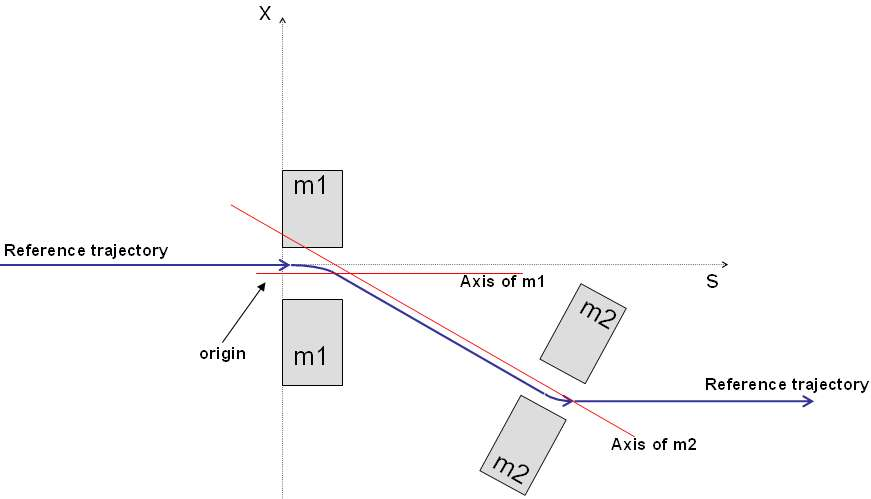
\includegraphics[width=450px]{Introduction/offsetelem.jpg}%%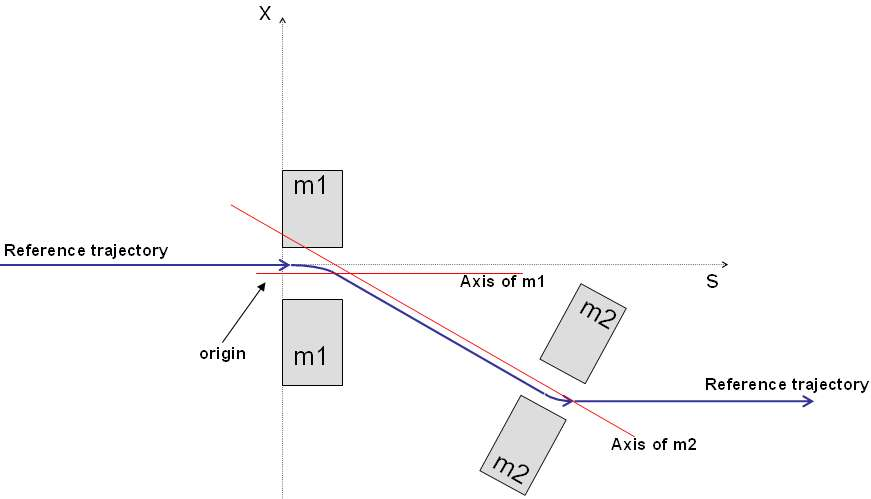
\includegraphics{offsetelem.jpg align=center width=780}
\\ The X\_ref(s) and Y\_ref(s) of the reference trajectory are calculated via an internal call to the \href{../survey/survey.html}{Survey} module. X\_offs(s) and Y\_offs(s) are derived from the coefficients given in the file. The resulting 
\begin{verbatim}
X_tot(s) = X_ref(s) - X_offs(s)\end{verbatim} and 
\begin{verbatim}
Y_tot(s) = Y_ref(s) - Y_offs(s)\end{verbatim} are taken into account in the aperture calculations.  
%%\begin{center}


\subsection{Aperture command example}
%%\end{center}

 The aperture module needs a Twiss table to operate on. It is important  not to USE another period or sequence between the Twiss and aperture  module calls, else aperture looses its table. One can choose the ranges  for Twiss and aperture freely, they need not be the same. 


\begin{verbatim}
use, period=lhcb1;
select, flag=twiss,range=mb.a14r1.b1/mb.a17r1.b1,column=keyword,name,
parent,k0l,k1l,s,betx,bety,n1;
twiss, file=twiss.b1.data, betx=beta.ip1, bety=beta.ip1, x=+x.ip1, 
y=+y.ip1, py=+py.ip1;
plot,haxis=s,vaxis=betx,bety,colour=100;

select, flag=aperture, column=name,n1,x,dy;
aperture, range=mb.b14r1.b1/mb.a17r1.b1, spec=5.235;
plot,table=aperture,noline,vmin=0,vmax=10,haxis=s,vaxis=n1,spec,
on_elem,style=100;
\end{verbatim}

 The \href{../Introduction/select.html}{select} command can be  used to choose which columns to print in the output file.  
\\ Column names: name, n1, n1x\_m, n1y\_m, apertype, aper\_1, aper\_2, aper\_3, aper\_4, rtol, xtol, ytol, s, betx, bety, dx, dy, x, y, on\_ap, on\_elem, spec 

 n1 is the maximum beam size in sigma, while n1x\_m and n1y\_m is the n1 values in si-units in the x- and y-direction. 

 aper\_\# means for all apertypes but racetrack:
\\ aper\_1 = half width rectangle
\\ aper\_2 = half heigth rectangle
\\ aper\_3 = half horizontal axis ellipse (or radius if circle)
\\ aper\_4 = half vertical axis ellipse

 For racetrack, the aperture parameters will have the same meaning as the tolerances:
\\ aper\_1 and xtol = horizontal displacement of radial part 
\\ aper\_2 and ytol = vertical displacement of radial part 
\\ aper\_3 and rtol = radius 
\\ aper\_4 = not used 

 On\_elem indicates whether the node is an element or a drift, and on\_ap  whether it has a valid aperture. The Twiss parameters are the interpolated  values used for aperture computation. 

 When one wants to plot the aperture, the table=aperture parameter is  necessary. The normal line of hardware symbols along the top is not  compatible with the aperture table, so it is best to include  noline. Plot instead the column on\_elem along the vaxis to have a  simple picture of the hardware. Spec can be used for giving a limit  value for n1, to have something to compare with on the plot. This example  provides a plot, 

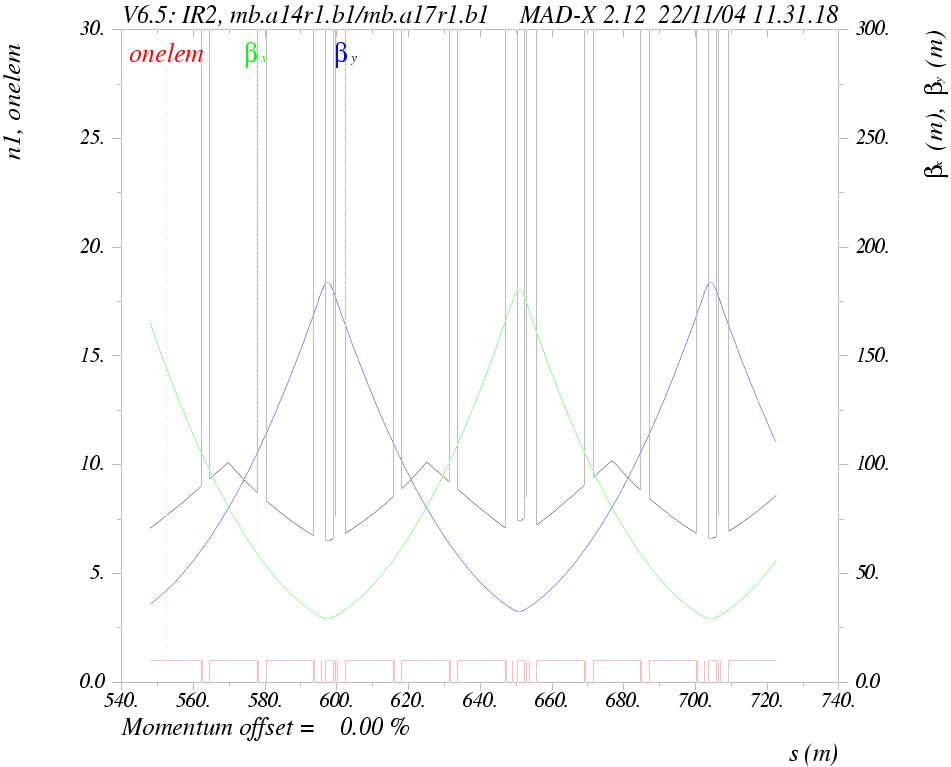
\includegraphics[width=450px]{Introduction/aperexample.jpg}%%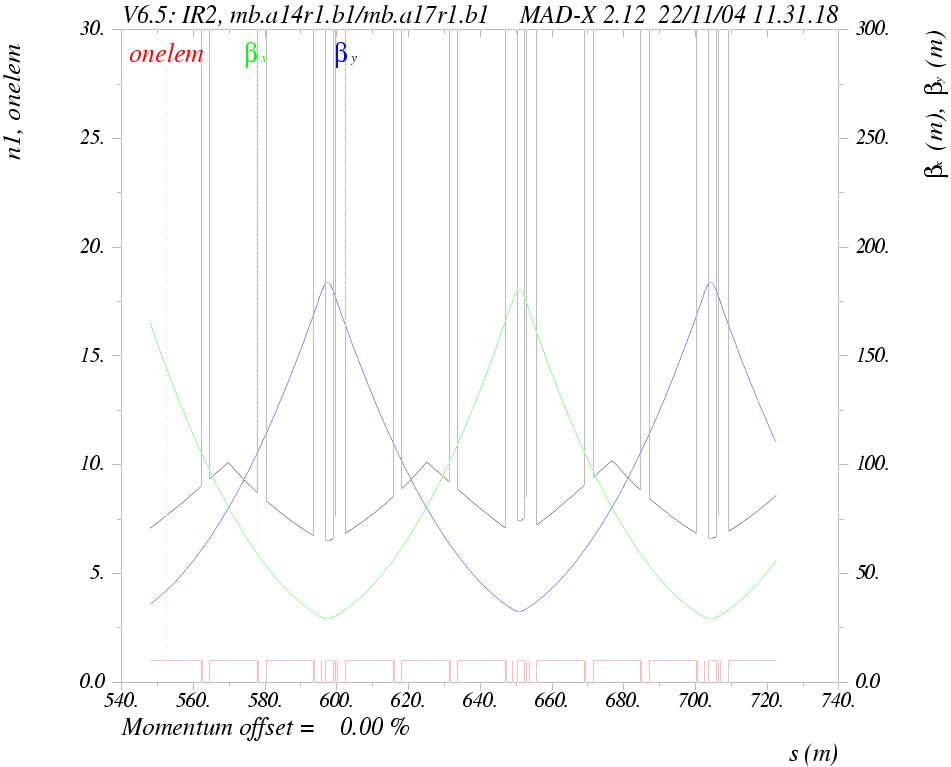
\includegraphics{aperexample.jpg align=center width=740}

 where we see the n1, beta functions and the hardware symbolized by on\_elem.    

\line(1,0){300}
\\
 Ivar Waarum, 24.02.05  -  Mark Hayes, 19.06.02 
\end{itemize}

%%\end{document}
